\documentclass{article}
\usepackage[utf8]{inputenc}
\usepackage{biblatex}
\usepackage{graphicx}
\usepackage{hyperref}
\usepackage{amsmath}
\addbibresource{references.bib}

\title{Markov State Models for Molecular Dynamics Protein Folding Simulations}
\author{Eric He}
\date{November 2019}

\begin{document}

\maketitle

\section*{Abstract}
The problem of protein folding is centered around understanding how the chain of amino acids comprising a protein folds into its stable, low-energy conformation. Because the laws of physics which govern the process are well-defined, protein folding can be simulated on computers. However, doing so requires a tremendous amount of computation and generates a large amount of folding data. 

This paper explains how to build Markov State Models to analyze protein folding data. As a form of probabilistic graph, Markov State Models can be used to process folding data generated from molecular dynamics data into a human-interpretable representation. Under the Markov State Model framework, protein folding is viewed as a probabilistic process rather than a deterministic one, and uncertainty around estimates can be quantified and used to focus simulation efforts to reduce the number of computations needed by two orders of magnitude.

Note: I did not realize the report was only meant to have 4 pages. Given this information, I decided it would be better to trim the survey to just the molecular dynamics section, since I believe depth is preferred to breadth.

\newpage
\tableofcontents
\newpage

\section{A brief introduction to the protein folding problem}

\begin{figure}
  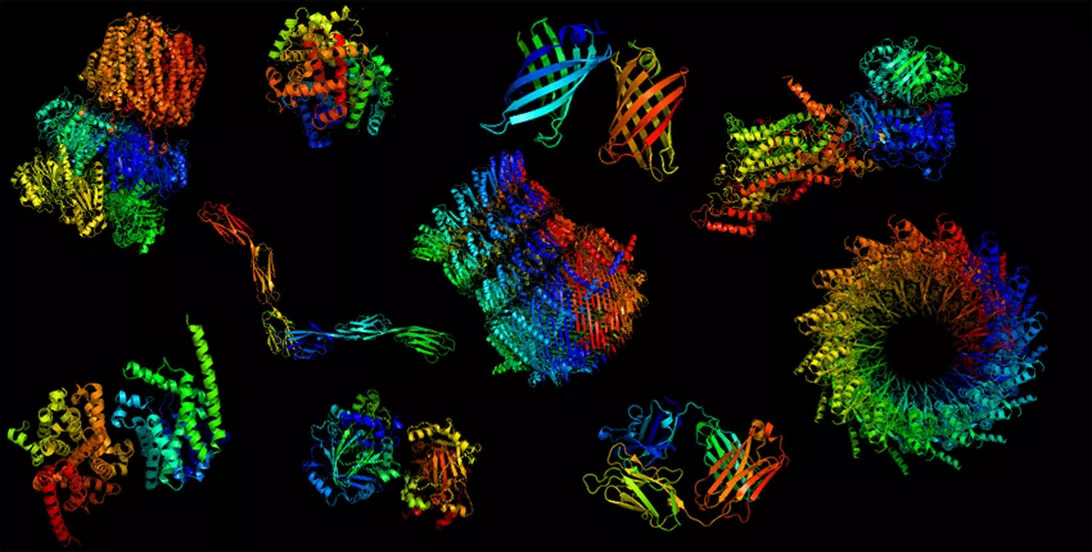
\includegraphics[width=\linewidth]{images/protein_folds.jpg}
  \caption{Examples of computer-generated protein folds by Mohammed Al-Quraishi}
  \label{fig:protein_folds}
\end{figure}

\subsection{The importance of protein folding}
Proteins govern nearly all biological processes, such as metabolizing food, transporting molecules, or providing structure to cells. A protein is created as a sequence of amino acid polymers, which \textit{folds} into a three-dimensional structure or \textbf{conformation} according to the physics of the amino acids comprising them and external forces such as water molecules or other proteins. For the vast majority of proteins, there is only one unique shape which the protein settles into, termed the \textbf{native conformation} or \textbf{native state}.

The native conformation determines a protein's ability to form chemical bonds with other molecules. In turn, a protein's chemical bonding properties determines its ability to perform its desired function; thus, it is commonly said that a protein's structure informs its function. The practical benefits of understanding a protein's native state include, but are not limited to:

\begin{itemize}
    \item modeling the dynamics of a protein's properties under mutations or misfoldings, especially in relation to diseases caused by malfunctioning proteins
    \item discovering drugs which allow us to control the activation or deactivation of target proteins
    \item identifying and tracing a protein's function through the course of its evolutionary history
\end{itemize}

Unfortunately, the minuscule size of proteins make it extremely difficult to map their structures. The only information of most known proteins are their amino acid sequences, derived from genomics data. Filling this gap is the goal of the protein folding problem. From a practical perspective, a mapping between a protein's sequence data and its corresponding structure would link what is known about a protein and what is needed to be known in order to usefully work with it. But more broadly, understanding protein structure provides the theoretical scaffolding needed to analyze biological systems as an emergent product of their underlying components.

\subsection{Physics underlying protein folding}
The protein folding process is governed entirely by physical laws. The primary ones are:

\begin{enumerate}
    \item The formation of hydrogen bonds between an amino acid residue with other residues in the chain, or the surrounding solvent
    \item van der Waals forces which attract or repel nearby atoms based on their electrostatic charges
    \item Chemical affinities towards the solvent, e.g. hydrophobia of certain molecules to water
\end{enumerate}

Many of the above forces are functions of temperature and acidity. Moreover, the presence of salts, folding catalysts, or \textit{molecular chaperones} can regulate the environment in which the protein folds.

Each of these forces push the amino acid chain towards conformations that lower the \textbf{Gibbs free energy}. The native conformation is typically attained when the free energy is globally minimized, but sometimes proteins can be trapped in a conformation which attains only a local energy minimum. Having proteins \textit{misfold} in such a manner is a known or suspected cause of many diseases such as Alzheimer's or Huntington's.

The vast majority of proteins fold at speeds on the order of nanoseconds to hundreds of milliseconds. Though quick on human timescales, this speed belies the complexity of simulating the process.

\section{Using Molecular Dynamics to simulate protein folding}
Since all physical laws governing protein folding are well-understood, computers can be used to simulate the protein folding process; this field is called \textbf{molecular dynamics} or \textbf{MD}. Unfortunately, simulations of the protein folding process require a tremendous amount of computing power to simulate the folding dynamics of even a single protein. 

The primary bottlenecks are the number of particle interactions involved and the amount of time steps to take. Though proteins fold in milliseconds ($10^{-3}$ seconds), simulations take timesteps on the order of femtoseconds ($10^{-15}$), requiring a quadrillion iterations to simulate a full second of folding \cite{md}. For each iteration, all interactions between atoms must be computed. This includes atoms belonging to the enveloping solvent, usually water molecules, which can be more numerous than the protein itself.

To sacrifice some accuracy in order to cut computational cost, MD simulations make various simplifications. \cite{md} gives some examples:

\begin{itemize}
    \item Electrostatic forces are simulated as point charges which might ignore effects such as the electric dipole moment.
    \item Stretching and bending of chemical bonds are modeled using harmonic functions instead of more accurate ones which model anharmonicity.
    \item Water molecules serving as solvent might be modeled as rigid or having a uniform temperature, or modeled only implicitly as a force field exerting random forces on the protein.
\end{itemize} 

\begin{figure}[ht]
  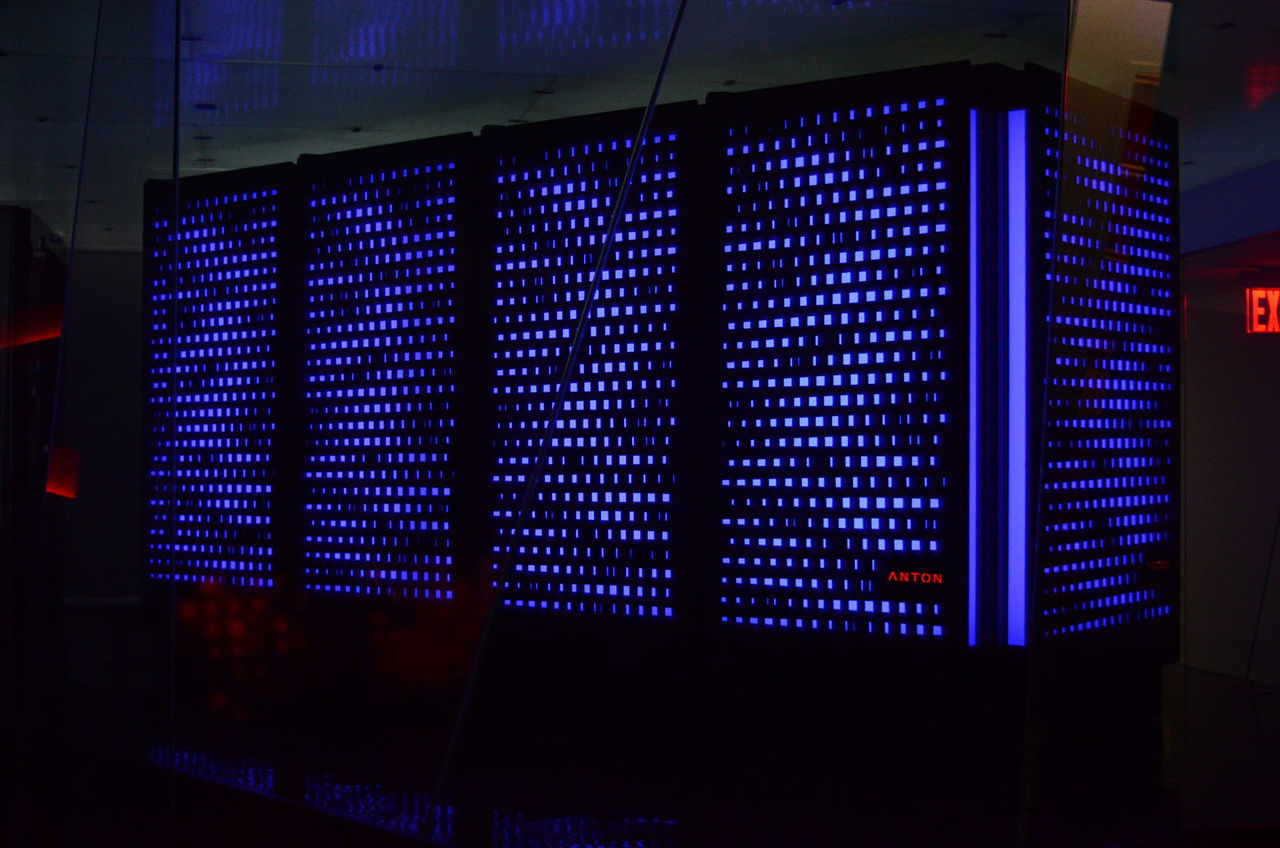
\includegraphics[width=\linewidth]{images/anton.jpg}
  \caption{Anton, a supercomputer built by D.E. Shaw Research specifically for protein folding computations. \cite{Anton} Photo by Matt Simmons}
  \label{fig:anton}
\end{figure}

Even with these speedups, MD simulations are still too slow to be useful purely for structure prediction. For example, a supercomputer purpose-built for protein folding computations, Anton, took around 100 days to simulate a single millisecond of the folding process for a protein comprised of around 1000 atoms \cite{Anton}.

\section{Markov State Models for interpreting data from MD simulations}
Despite their suboptimal use for structure prediction, MD simulations are still valued because they depict the folding process itself. Apart from being theoretically important, this is also of special interest in the study of diseases which are caused by proteins misfolding away from the standard resting conformation; some examples where misfolded proteins are the suspected cause of a disease include Alzheimer's and Huntington's.

To understand folding trajectories of a protein, it is not enough to simulate a single fold of the protein. Instead, a protein's folding process must be simulated many times to derive an understanding of the probability space over the protein's possible conformations. As a result, scientists working on large MD simulations must be able to both gather and comprehend vast amounts of time series data of a protein's probable conformation. 

A ubiquitously used tool in MD, popularized by the Pande lab at Stanford is the \textbf{Markov State Model} or \textbf{MSM} \cite{pande2010}. MSMs group \textit{clusters} of conformations into states of a Markov chain; the folding process is viewed probabilistically as walking through states of the chain until reaching an absorbing state corresponding to the resting conformation. MSMs grant the ability to:

\begin{enumerate}
    \item Group together similar conformations into human-comprehensible clusters
    \item Map which folding pathways are most favored by the protein
    \item Adaptively sample conformations contributing high uncertainty to relevant metrics (such as the folding rate of the protein) to save computation time
\end{enumerate}

We begin with an intuitive example of MSMs, then explain how to construct and quantitatively analyze an MSM.

\subsection{An example of an MSM}

\begin{figure}[!h]
  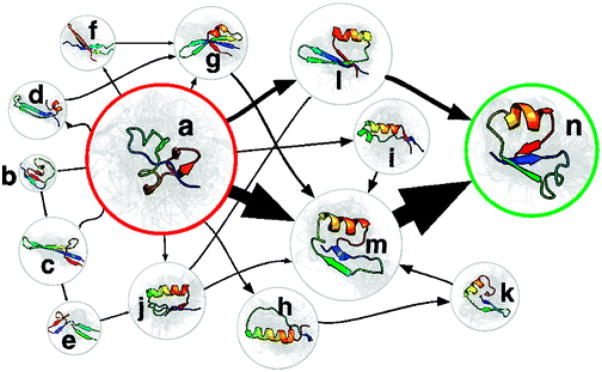
\includegraphics[width=\linewidth]{images/folding_pathways.jpg}
  \caption{Different probable states of a protein fold derived by learning a Markov State Model on Molecular Dynamics simulations in \cite{pande2010}}
  \label{fig:foldingPathways}
\end{figure}

Mathematically, the MSM is parameterized by a macrostate-macrostate transition matrix $T$, where the $i,j$th entry $T_{i,j}$ represents the probability of transitioning to macrostate $j$ while in macrostate $i$. 

Each macrostate is comprised of a multitude of \textit{microstates}, themselves smaller clusters of conformational space. While the microstates are clustered according to \textit{structural} distances measuring how far apart two conformations are in physical space, the macrostates cluster microstates based on \textit{kinetic} distances measuring how frequently two conformations transition between each other during folding. 

This hierarchical clustering is performed because while the ideal clusters should group together conformations which are close in free energy space, mapping free energy space is extremely difficult from both a computational and theoretical perspective. Thus, structural and kinetic distances are mixed together as an approximation to free energy space. 

\autoref{fig:foldingPathways} gives us a pictorial depiction of an MSM. Each node represents a supercluster of conformations termed a \textit{macrostate}, with the relative size of the node being proportional to the expected time spent in that cluster. The directed edge $x \to y$ from two arbitrary macrostates $x$ and $y$ in the MSM is shown as an arrow, with the arrow's relative size being indicative of the speed and/or relative likelihood of transitioning to state $j$ from state $i$.

The protein starts in state $a$, bordered in red, and eventually folds into the resting conformation at state $n$, bordered in green. The most direct and commonly used path is directly through state $m$, but in some situations the protein was shown to detour through states $b, c, e,$ and $j$ before reaching $m$. Rather than just considering one or two folding trajectories, MSMs generate probability distributions over folding pathways, which can be sampled by stepping through the macrostate's transition matrix, then emitting a microstate based on the particular macrostate sampled, much as in a Hidden Markov Model. 

\subsection{Constructing the MSM}
\subsubsection{Clustering microstates using a modified $k$-means algorithm}
The first step in constructing an MSM is deciding how to create the aforementioned \textit{clusters} of conformations. We walk through an approach implemented by the Pande lab in their `MSMBuilder` \cite{msmbuilder} software package is a variation of the k-means clustering algorithm in which centers for new clusters are iteratively initialized to occupy the point furthest from all the existing cluster centers \cite{pande2009}. This variation of k-means encourages clusters to have roughly equal radii. The metric used for this clustering algorithm is a \textit{structural} (rather than kinetic) distance between two conformations known as \textit{Root Mean-Squared Deviation}, or \textit{RMSD}.

This methodology is used to create fine-grained clusters, termed \textit{microstates}. Typically between $10,000$ and $100,000$ microstates are created. 

\subsubsection{Computing the microstate transition probability matrix $T$}
The transition probabilities between microstates $i$ and $j$ can be naively computed as the \textit{maximum likelihood estimate} (MLE), corresponding to the number of times state $i$ transitioned to state $j$, divided by the total number of transitions from state $i$ to other states $k \neq j$ (including $k=i$). If $C_{ij}$ corresponds to the $i,j$th entry of a \textit{count matrix} tabulating the number of times state $i$ transited to state $j$, the MLE is given the formula

$$T_{ij} = \dfrac{C_{ij}}{\sum_k C_{ik}}$$

The MLE, however, can lead to noisy estimates for sparsely sampled microstates. Moreover, it might not satisfy the property of \textbf{detailed balance}, a kinetic property of systems at equilibrium stating that the average rate of transition from state $i$ to state $j$ is equal to the average rate of transition from state $j$ to state $i$. A Markov chain is said to be reducible or to have detailed balance if the following equation is satisfied for arbitrary states $i$ and $j$:

$$\pi_i T_{ij} = \pi_j T_{ji}$$

\noindent where $\pi_i$ is the stationary probability of being in state $i$.

Thus, a more principled way of estimating the transition probabilities is to restrict the space of Markov chains to the ones satisfying detailed balance. A closed-form solution for the MLE reversible Markov chain $X$ in this space is given by the following equation:

$$T_{ij} = \dfrac{C_{ij} + C_{ji}}{\frac{C_i}{T_i} + \frac{C_j}{T_j}}$$

According to \cite{pande2009}, this method works well for small MSMs, but takes time to converge for larger matrices and can see poor performance when the MD simulation is noisy. 

Given the microstate transition matrix $M$, kinetic relationships can be used to further cluster microstates into macrostates. This can be done by looking at the dominant eigenvectors of $M$. One method, known as \textit{Perron Cluster Cluster Analysis} or \textit{PCCA}, partitions microstates into \textit{meta-stable} macrostates by finding a grouping such that the corresponding macrostate transition matrix $T$ of specified size $d$ has the largest possible trace \cite{fishbach}. Having the largest trace indicates that each macrostate groups together as many kinetically similar microstates as possible, since inter-state transitions are small.

\subsubsection{Incorporating Bayesian priors over MSM parameters}
A powerful, but computationally demanding way to evaluate estimations of the macrostate-macrostate transition matrix $T$, the macrostate-microstate emission matrix $\Theta$, and the choice of macrostate clustering or \textit{lumping} $L$ is given in \cite{msmprior}. 

The method is to further impose priors on the macro and microstates and use those priors to compute \textit{Bayes factors}. The Bayes factor is a ratio of two posterior probabilities; since the posterior factors in the prior, complex models are penalized by the Bayes factor since even they have a lower prior probability; thus, to be accepted over a simpler model, a more complex model must have a sufficiently higher likelihood. The recommended methodology is as follows:

\paragraph{The prior over $\Theta$} is a Dirichlet prior. The emissions probability for a state $theta_j$ follows a Multinoulli distribution, whose conjugate prior is Dirichlet. 

\paragraph{The prior over $T$} can also be a Dirichlet prior over stochastic matrices, but from the previous discussion, a better prior is the Dirichlet prior restricted to the space of stochastic matrices satisfying detailed balance. The density has a closed form solution, but the formula is quite complex. The derivation is found in \cite{diaconis}.

\paragraph{Selecting $L$ using Bayes factors} The optimal $L$ for a certain macrostate size $d$ can be found using PCCA or its more robust variants, PCCA+ and PCCA++. Given two such choices $L_1$ and $L_2$ from the data $D$, the Bayes factor can be computed as the ratio of the posteriors

$$\dfrac{P(L_1 | D)}{P(L_2|D)} = \dfrac{P(D|L_1)}{P(D|L_2)}\dfrac{P(L_1)}{P(L_2)} 
= \dfrac{\int_T \int_\Theta P(D|L_1, T, \Theta)P(T, \Theta | L_1)}
{\int_T \int_\Theta P(D|L_2,T,\Theta)P(T, \Theta | L_2)}$$

Interpreting the Bayes factor is straightforward. If the Bayes factor is less than $1$, then $L_2$ should be preferred over $L_1$. If the Bayes factor is greater than $1$, then $L_1$ should be preferred to $L_1$. If the priors over $T$ and $\Theta$ are both Dirichlet, then an analytical solution for the Bayes factor can be given. Using the detailed balance Dirichlet prior for $T$, however, requires Monte Carlo integration.

\subsection{Validating the Markovian properties of an MSM}
An MSM makes the fundamental \textit{memoryless} or \textit{Markovian} assumption that our expectation of future states is independent from the knowledge of past states when conditioned on the present; that is, information on the current conditions of a protein is all that is needed to forecast its future folds. This assumption is fundamentally correct for individual conformations, but improper aggregations of conformations can violate the Markov assumption.

\subsubsection{A non-Markovian aggregation of states}
A straightforward example of an improper aggregation would be aggregating states $c$ and $m$ in \autoref{fig:foldingPathways} into a hypothetical superstate $o$. The Markovian assumption would say that given the protein is in superstate $o$, no further information is needed to predict the future folding trajectory. However, if the protein transitioned into state $o$ from state $b$, it is highly likely that the protein will go towards states $e$ or $b$ or $a$, since the protein is actually in state $c \in o$. On the other hand, if the protein entered state $o$ from state $a$, it is almost certain to be in state $m \in o$ and therefore is almost certain to transition to the resting conformation $n$.

The superstate $o$ thus exhibits non-Markovian properties, since its transition probabilities are largely a function of what state the protein was in previous to $o$, rather than depending solely on $o$ itself.

\subsubsection{Geometrically distributed leaving times}
The Markovian assumption implies strong distributional effects which can be cast as statistical tests for empirical verification. One such test observes that for a candidate transition matrix $T$, the expected amount of time a fold remains in a specified state $i$ follows a geometric distribution. The geometric distribution parameter $p_i$ for state $i$ corresponds to the probability of remaining in state $i$ upon experiencing a pass through $T$; this is simply $T_{i,i}$. If the empirical leaving times are not distributed according to their corresponding geometric distributions, this is a strong indication of non-Markovian dynamics.

\subsubsection{The Swope-Pitera eigenvalue test}
Another test is the \textbf{Swope-Pitera eigenvalue test} described in \cite{swopepitera}, which examines the magnitude of the eigenvalues of the transition matrix $T$ compared to the eigenvalues of $T^n$. 

To establish the foundations of the Swope-Pitera test, some of the spectral properties of aperiodic and irreducible Markov chains must first be presented. Such a Markov chain has all eigenvalues but one less than $1$, with this last eigenvalue being equal to $1$ (\textit{unity}). An eigenvector with eigenvalue $\mu$ represents a state distribution which decays towards the stationary distribution at rate $\mu^t$ where $t$ is the number of transitions through the transition matrix $T$. Thus, the states with larger eigenvalues decay more slowly, while the eigenvector corresponding to unity represents the state which does not decay, the stationary distribution itself. The eigenvectors of the matrix $T^t$ are equivalent to the eigenvectors of $T$, with the corresponding eigenvalues $\mu_t = \mu^t$.

The Swope-Pitera test evaluates whether the eigenvalues of an empirically constructed matrix with timestep length $t$ are exponentially decaying as expected. That is, the eigenvalues $\{\mu_t\}$ of the length-$t$ transition matrix $T_t$ should be roughly equivalent to $\{\mu^t\}$, where $\{\mu\}$ is the set of eigenvalues of the length-$1$ transition matrix $T_1$. Lack of exponential decay is an indication of non-Markovian dynamics.

\subsection{Adaptive Sampling with an MSM}
Given an MSM, it is possible to estimate quantities such as the \textit{mean first passage time}, which corresponds to the expected time a conformation takes to fold. Importantly, we can also compute our uncertainty around these estimates and even identify which states are contributing the most variance. This provides a critical advantage, since by upsampling or \textbf{adaptively sampling} these uncertainty-contributing states, sufficiently low uncertainty can be achieved using orders of magnitudes less simulation steps, according to \cite{pande2010}. The adaptive sampling method discussed here comes from \cite{adaptivesampling}.

\subsubsection{Estimating a distribution for the states of $T$}
To measure the uncertainty of metrics such as mean first passage time, we must first measure the uncertainty of the underlying transition probabilities. Recall that the distribution of transition probabilities for $T$ is a Multinoulli. Since the Multinoulli's true parameters are unknown, we assume a distribution over possible Multinoulli distributions using the conjugate prior, the Dirichlet distribution.

If the prior over the Dirichlet parameters is the vector $\boldsymbol{\alpha}$ and the empirical transitions form the counts $\boldsymbol{z}$, then the posterior distribution is given by a Dirichlet with parameter $\boldsymbol{\mu} = \boldsymbol{\alpha} + \boldsymbol{z}$.

Directly using the Dirichlet distribution for sampling transitions in $T$ is computationally expensive, so the distribution is approximated using a multivariate normal distribution or \textit{MVN}. A Central Limit Theorem justifies the approximation with the statement that the Dirichlet distribution approaches a Multivariate Normal distribution as the number of samples goes to $\infty$. 

Specifically, for a specific state $i$, as the vector of Dirichlet counts $\boldsymbol{\mu_i}$ has magnitude $w_i = |\boldsymbol{\mu_i}| \to \infty$ and as $\dfrac{\boldsymbol{\mu_i}}{w_i} \to \boldsymbol{v_i}$ for some fixed probability distribution $\boldsymbol{v_i}$, the Dirichlet distribution parameterized by $\boldsymbol{\mu_i}$ converges pointwise to a Multivariate normal distribution with parameters $\boldsymbol{\mu_{\text{norm, i}}} = \dfrac{\boldsymbol{\mu_{\text{dir, i}}}}{w}$ and covariance matrix $\boldsymbol{\Sigma_i} = \dfrac{1}{w_i(w_i+1)}(w_i\mu_i - \mu_i\mu^T_i)$.

\subsubsection{Monte Carlo estimation of a target metric's variance}
The transition matrix $T$ allows the deterministic calculation of relevant metrics. One example is the \textit{mean first passage time}, the expected amount of time it takes a given conformation to fold into the resting conformation. The formula for mean first passage time $x_i$ of state $i$ given the transition matrix $T$ is as follows:

\begin{equation*}
    x_i =
    \begin{cases}
    \Delta t + \sum_{j=1}^K x_jT_{ij} & i \neq K \\
    0 & i = K
    \end{cases}
\end{equation*}

\noindent where $K$ is the row of $T$ corresponding to the resting conformation.

Frequently we are also interested in our uncertainty around these metrics. Note that this uncertainty is a concept separate from the natural variance of the metric; the former is an estimate of our lack of knowledge based on the Dirichlet distribution of each row in $T$, while the latter is an estimate of the actual variance in folding time based on the hypothetical true Multinoulli distribution of each row in $T$. 

The variance of the Dirichlet distribution around a particular row can be reduced by generating more samples of the corresponding state, but the variance of the Multinoulli is a fixed constant. Thus, when we discuss reducing variance, we are talking about reducing the variance of our Dirichlet estimate of the true Multinoulli distribution rather than the variance of the Multinoulli itself.

When a formula for the uncertainty of a target metric is intractable or inconvenient to compute, it can be estimated by generating random draws from the corresponding rows of $T$, or their MVN approximations, to create Monte Carlo samples of the target metric from which the uncertainty can be estimated. 

For many metrics, this formula for the uncertainty cannot be decomposed into a sum of the variances of individual rows of $T$ unless a first-order Taylor approximation of the metric is performed. This approximation reduces the formula to a set of linear equations with easily solvable, closed-form solutions.

\subsubsection{Targeted sampling to achieve minimal variance}
Given an estimate of variance of the target metric which can be decomposed into the contributions of the individual rows of $T$, it is straightforward to design an adaptive sampling algorithm to reduce this variance. 

Given a fixed number of additional samples $m$ to generate, states should be ranked in descending order of their expected change in variance by adding those $m$ samples. Then $m$ simulations starting from microstates within state $i$ can be started. 

The results of these $m$ simulations can be used to recompute the estimate of $T$ and determine the next state to simulate $m$ times.

\section{Conclusion}
MSMs are a critical auxiliary method for protein folding molecular dynamics research. By grouping conformations into a hierarchical microstate and macrostate representation, MSMs provide high-level summaries of the distribution of possible protein folding trajectories. By being able to quantify and attribute uncertainty to individual states, MSMs allow focused simulations which converge to the required confidence level two orders of magnitude faster than naively repeating simulations.

\printbibliography

\end{document}
